%%%%%%%%%%%%%%%%%%%%%%%%%%%%%%%%%%%%%%%%%%%%%%%%%
%%%%%%%%%%%%%%%%%%%%%%%%%%%%%%%%%%%%%%%%%%%%%%%%%

\chapter{Foraging}
\label{chap:second}

%%%%%%%%%%%%%%%%%%%%%%%%%%%%%%%%%%%%%%%%%%%%%%%%%
%%%%%%%%%%%%%%%%%%%%%%%%%%%%%%%%%%%%%%%%%%%%%%%%%

%The same structure as before, including section, subsections and sub-subsections. Make sure that you follow the same conventions throughout, to avoid confusing the reader. Always remember to include a summary.

%%%%%%%%%%%%%%%%%%%%%%%%%%%%%%%%%%%%%%%%%%%%%%%%%
%%%%%%%%%%%%%%%%%%%%%%%%%%%%%%%%%%%%%%%%%%%%%%%%%

\section{Definition}
\label{sec:second:definition}

In swarm robotics, robot foraging has become a benchmark problem due to its complex nature involving the coordination of numerous sub-tasks. The problem was initially addressed by biologists, particularly in the foraging behaviour of ants \cite{holldobler1990ants,bernstein1974seasonal}, bees \cite{seeley2009wisdom} and bacteria \cite{resnick1994turtles}. Foraging has a variety of real-life applications such as search and rescue \cite{jennings1997cooperative,murphy2000biomimetic}, and waste clean-up \cite{balch1995io}. Numerous swarm robotics algorithms have been developed to improve robustness, time and energy efficiency of the foraging process for multiple variations of the foraging problem as outlined in \cite{winfield2009foraging}. 

Foraging is the act of searching for and collection (or capturing) food for storage and consumption \cite{winfield2009foraging}. Foraging is an important problem that was first addressed by biologists in the examination of nature, particularly with the foraging behaviour of ants and bacteria. In a robot context, foraging is defined as the search and collection of scattered objects in an environment and returning those objects to a collection point.

The foraging sub-tasks involve the efficient search and collection of food, homing whilst carrying food to the nest site and then deposition of the food item in the nest before returning to foraging. Effective foraging requires co-operation using signals or direct cooperation of individuals in order to transport food items too large for individual transport.  

%Naive foraging?? Probably save for later. 
A basic finite state machine foraging model, has four states: Searching, grabbing, homing and depositing. A foraging robot is always in one of these four states. There is a single collection point or nest and that there are more than one target objects. The process is continued indefinitely until all objects are foraged. The states are defined as follows:

\begin{itemize}
\item Searching: requires physical movement. It is assumed that a robot cannot locate and retrieve items by remaining in a single position due to sensors, physical limitations and environmental occlusions.
\item Grabbing: is the physical seizure of an item in order to transport it back to the nest. The model assumes the object can be grabbed by a single robot.
\item Homing: is the movement to the nest with the collected object. This step has three stages. Initially, the position of the nest relative to the current position must be determined, followed by determining the orientation of the robot towards the position of the nest. Lastly, actual navigation towards the nest via odometry to retrace robots steps or using long range homing beacons. 
\item Depositing is the deliverance of the object to the nest and the state transitions back to searching 
\end{itemize}

The basic foraging process has been adapted for numerous foraging problems and for different types of robots and is often replaced completely with more complex models, including communication components and division of labour.

\section{Biological Inspiration}

As with most swarm robotics problems, the inspiration comes from nature - in particular, social insects such as Ants and Honeybees. This chapter describes the biological models that are used in the algorithms derived by this thesis. 

\label{sec:second:biological}

\subsection{Ants}
%Ants
The study of ants has revealed that impressive emergent activities can be achieved with  simple agents with few very simple rules. As a result, the pheromone foraging behavior activities of ants have been modelled in swarm intelligence \cite{dorigo2006ant, dorigo2010ant}. Ants use a form of communication known as stigmergy \cite{} where ants deposit a substance known as pheromone on the paths between the nest and the food source. Other ants can detect this pheromone and will tend to follow paths which have greater amount of pheromone deposits. 

The desert ant (\textit{Cataglyphis bicolor}) does not make use of pheromone-based communication to forage, as pheromone deposited on desert sand would be blown away by the wind. Instead, desert ants use a technique called path-integration for navigation to relocate food sources that have already been found by random exploration \cite{collett1998local}. 

An overall heading and distance from the nest is maintained as the desert ant explores. As a result, a shortcut back to the nest is calculated in order to minimize heat stress. This is a key evolutionary aspect gained from living in the hot barren desert. The path integration navigation does not depend on the existence of landmarks, making it suitable to any type of environments. 

Although algorithms based on ant foraging behaviour are used to solve optimization problems, the algorithms are often difficult to replicate in a real-life robotic environment as many of the techniques conceptually use pheromones.  A robotics algorithm that uses pheromone either requires robots to be equipped with a substance-distributor, beacon-deployer or a complex simulation of pheromone, requiring communication \cite{hoff2010two}.


The desert ant is thus simpler to model for real-robot interaction. Desert ant foraging has been modelled and experiments have been performed on real robots in \cite{hecker2012formica}. Experiments were performed using a small set of robots in a small arena on different environment types. Two algorithms were evaluated: one based on the desert ant foraging and one including pheromone-like communication. It was shown that communication improved performance; however, the desert-ant algorithm still performed reasonably. 


\subsection{Honey bee}

Honey bee foraging is made up of three different roles \cite{seeley2009wisdom}: Employed foraging, unemployed foraging and scouting. Scouts explore the environment to locate new food sources. Once a source has been found, scouts return to the hive to communicate information about the located food source. To communicate foraging information, scout bees perform a waggle-dance on the hive, containing information about the distance and bearing of the resource. Communication of good foraging sites is known as recruitment. 

Unemployed foragers wait on the dance floor, evaluating the dances of the scout bees. An  unemployed bee chooses a location described by the scout bees, and becomes an employed forager. Employed forager bees use the information about the resource, attempt to locate the source, load themselves with food and return to the hive where unemployed foragers are ready to offload the food. Jansen \cite{janson2007searching} suggests that unemployed bees become exploring scouts when they do not detect any dancing scout bees. 

Bee swarms have been used in swarm robotics for problems such as path planning \cite{lin2009chaotic}, aggregation \cite{kernbach2009re}, collective perception \cite{schmickl2007collective}. 


%%%%%%%%%%%%%%%%%%%%%%%%%%%%%%%%%%%%%%%%%%%%%%%%%

\section{Taxonomy of Robot Foraging}
\label{sec:second:taxonomy}

Foraging is a popular problem due to its vast opportunity for application. The problem has been adapted into many different variations in order to cater for the different environments and applications that foraging can be applied to. It is thus beneficial to present a taxonomy of robot foraging that can be later used to classify the specific foraging problem being addressed by this thesis. Multiple taxonomies have been developed as robot foraging research has progressed \cite{oster1978caste,ostergaard2001emergent}. Winfield presents and discusses a very complete foraging taxonomy which classifies foraging solutions based on characteristics of four major axes: the foraging environment, robots used for foraging, performance aspects and the foraging strategy used. Each of these major axes have a number of minor categories which are outlined in the table below.  

\begin{tabular}{l | c | r }
	\hline
	Major Axis & Minor Axis & Value  \\ \hline
	\multirow{3}{*}{Environment} & Search space & Unbounded \\ 
	& \multirow{2}{*}{Source Areas} & Unbounded \\ 
								& Constrained \\
	& Sinks & Unbounded \\
	& Object types & blergh \\
	& Object Placement & blergh \\
\end{tabular}

Give a brief overview of existing ones. Go dig up those papers. 
Outline my own taxonomy and why it is different. Multiple taxonomies for classification of robot foraging algorithms exist. The latest and most complete is that of [citation].

%Outline the 

%%%%%%%%%%%%%%%%%%%%%%%%%%%%%%%%%%%%%%%%%%%%%%%%%

\section{Existing Foraging Solutions}
\label{sec:second:existingsolution}


%This section discusses some foraging solutions that have been developed as well as looks at the different types of foraging problems. 

%Mention the current attempts at foraging. 
%Keep in mind to mention the papers about the techniques that I am comparing. 
%The desert ant, bee techniques, basic ones. 
%Mention but don't go into details about papers that attempt very specific ones.
%Insect Inspired
%----------------------------
Insects are used as inspiration throughout swarm robotics due to there roboust and flexible swarms. Ants utilize pheromones which is a robust strategory for local interactions and would prove useful in hazardous environments. 
%citation & write better.

%Blazing a trail => Nice paper - need to discuss more. Maybe in navigation
Vaughan presents a swarm robotic algorithm allowing for robust transportation of items from a single source to a single sink in an environment with spatial constraints \cite{vaughan2000blazing}. The algorithm presented makes use of both ant-like and bee-like foraging techniques. The ants broadcast the landmarks in the area for odometric localization as well as uses a form of the  honey bee "waggle dance" that communicates the direction of the food source from the robot that has found the food source to other robots. The robots use a technique called path integration utilized by both ants and bees in order to maintain position and heading estimate. Using these techniques the robots communicate multi-segment paths. These communications occur globally. This technique suffers from accumulation of localization errors over time due to the use of global communication. Local communication is preferred for the algorithms developed in this study.   %Our robot algorithms can reaign the sink %citations required!!!! %necessary? Worth a mention. 

%Fotan & Mataric
Schneider \cite{schneider1998territorial}, in order to reduce the interference caused by collisions, develop an algorithm to split the foraging environment into bounded areas for which a robot is in charge of. The sink area of one robot is the source area for the next, resulting in the emergence of bucket brigading behaviour. The bucket brigading algorithm is not suitable to environments where the size of the environment is not known - unless an algorithm is developed that will effectively allow a swarm of robots to divide the area. The algorithm is thus not suitable for comparison for the current study. The failure of a robot induces readjustment of territories in order to effectively cover the foraging area. Global information about the environment is used and as a result the algorithm is not suitable for comparison. %Reread to figure out if initial distribution algorithm exists

%Mataric
\O stergaard \cite{ostergaard2001emergent} determines that there is a finite number of any particular type of robot that is optimal for performing a foraging task. Mataric compares the algorithm to a naive algorithm which represents the baseline foraging task with no improvements. The naive algorithm in the thesis as a baseline comparison measure and is discussed in more detail in further chapters. Mataric found that if too many robots were allocated to the environment then extreme amounts of interference occurred which decreased the performance of the algorithm. Emergent bucket brigading was shown to perform better than naive in highly constrained environments however naive performed better in open environments. Algorithms are tested in environments of differing difficulties. %Need to read this paper to check which one these details came from. Also DO the thing for his name


%Goldberg + Mataric
Goldberg and Mataric \cite{Goldberg01designand} address the foraging problem with multiple sources and sink areas in an open field environment. The study focuses on interference reduction by making use of a dominance hierarchy - only the dominant robot near the sink can take an item to the sink. %mentioned PACK foraging. read up

%Mataric and Werger
Mataric \cite{werger1996robotic} and Werner discuss produced an algorithm where chains of robots are formed and the robots forage in circular excursions. The length of the change is then adusted according to the amount of food found by the foragers. %No idea how this works - read up. 
 
%Swarming Robots: Foraging Behaviour of Simple Multi-Robot System
Sugawara \cite{sugawara2002swarming} implements a foraging solution for a single food source. The algorithm is based on naive foraging however utilizes simple communication. A robot will stay and broadcast a light signal on finding an item. Other robots are attacted to the light signal based on an angular velocity equation. This differs from the techniques used in this thesis as all food sources communicated with equal weight where as the quality of a food source is evaluated by the honey bee algorithm.

%Alexandre Campo 2006 - Efficient multi-foraging robotics
\subsection{Multi-foraging}
Multi-foraging is defined as a type of foraging problem where instead  multiple object types are required to be foraged. \cite{Balch99rewardand}. The types of objects can have different characteristics and can be collected together or separately.



%Adaptive DoL in Large-scale Minimalist MultiRobot systems - Mataric.
%2 types of items 
Jones et al \cite{jones2003adaptive} describe a version of the problem where there exist two types of items and items are consumed instead of transported to the sink and as items are consumed, the same type of item is placed at a random spot in the arena. Robots signal what type of item they are foraging by a coloured light which other robots use to build a local history of the number of robots they have seen that are allocated to each item type. A history of the number of observed items of each type is also collected. The division of labour capability is formed by estimating the current division of labour of the group by  using the described local observations. The estimations are then used to determine the probability of changing from foraging the current item type to the other type. 

%\begin{equation}
% P(Green - Red) = \left\ {
%	\begin{array} {l l}
%		(GR - GP_*(1-GP) & \quad \textrm{if GR \geq GP} \\
%		0, & \quad \textrm{otherwise}
%	\end{array}
% \right.
%\end{equation} 

%		(RR- RP)*(1-RP) & \quad \text{if RR $\geq RP$
%%%%DoL$
Campo \cite{campo2007efficient} performs a study in order to identify characteristics of efficient multi-foraging behaviour.  A mathematical model is developed and validated to predict optimal foraging behaviour and thus allows absolute evaluation of the proposed decision algorithm. The proposed foraging decision algorithm utilizes the amount of other robots encountered as well as the amount of prey encountered to only allocate enough robots foraging  so that remaining robots can spare energy. A measure is proposed that estimates the instantaneous energy that a robot group can gain, which each robot uses to guide the search process. 
%Need to add discussion
%Says prey

Balch \cite{balch1999impact} develops a technique for multi-foraging and determining the impact of robot diversity on multi-foraging performance. This thesis's does not consider robot diversity since robots are homogenous.
  
  
\section{Nature-inspired Algorithms}

%%%%%ANTS%%%%%
Hoff \cite{hoff2010two} classifies different types of ant-inspired pheromone-based foraging algorithms by the way pheromones are represented: physical marks \cite{alcoholfromants2012}, use of existing communication channels such as sharing over wireless networks as well as virtual pheromone. %Read further

%DoL in a Group of Robots Inspired by Ants Foraging Behaviour - Labella + Dorigo
Labella et al \cite{labella2006division} propose a foraging model inspired by the foraging of ants, where individual robots adapt to the environment using only locally available information. The adaption allows for effective division of labour to occur. The probability $p1$ that a robot will changed from rest to searching is adapted upon return to the sink and from deposit to rest. If a robot fails to forage any prey after searching for a specified maximum time, then the robot returns and rests. 
The adaption rule increases or decreases $p1$ by a constant $\Delta$ that is multiplied by the number of consecutive successes or failures. The study showed that adaption improved the amount of time spent not at rest. The advantage to this type of algorithm is its simplicity as no communication is required to regulate the number of robots. As pointed out, there is a global negative effect on overall efficiency at large group sizes. This is to be expected, but is not a serious problem since less energy is used, and this would be an advantage when energy is a scarce resource. %rephrase%
%Different from the problem proposed in this study as different priorities of items are not considered
%Come back and do a bit later. 
%Says prey

\begin{figure}
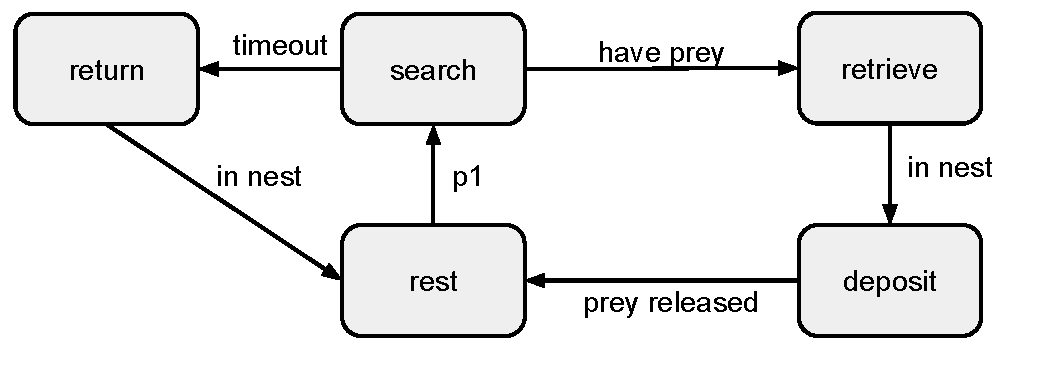
\includegraphics[width=\textwidth]{chapters/chapter2/figures/LabellaFSM.pdf}
\caption{Simplified finite state machine for Labella division of labour algorithm. }
\end{figure} 

Hoff \cite{hoff2010two} proposes a two ant-based foraging algorithm which do not require marking the physical environment. Instead, robots themselves become pheromone markers. The algorithms differ in the manner in which the beacon-to-pheromone role is chosen. 

Virtual pheromone algorithm functions as follows: Two pheromone trails are created - one trail from the source to the food and another trail from the source to the nest. The trail is created by robots: During execution, robots stop exploration and become pheromone beacons. The pheromone beacon robots simply broadcast a floating point number known as virtual pheromone. 
Local direct communications are used to transmit the virtual pheromone value.

The second technique uses cardinality where if a robot can hear 2 or more beacons then the robot stays a walker else the robot becomes a beacon. %Etc etc add more from paper!!!!


The advantage of using this technique over the other mentioned pheromone techniques is that robots are simpler due to simpler communication mechanisms as well as the lack of need for complex beacon deployment systems. Experiments are conducted with and without obstacles and a real-world simulator is used. The result show that congestion effects performance the most at high robot density. %write more in more detail. The cardin







%%%%%%%%%%%%%%%%%%%%%%%%%%%%%%%%%%%%%%%%%%%%%%%%%
%%%%%%%%%%%%%%%%%%%%%%%%%%%%%%%%%%%%%%%%%%%%%%%%%


\section{Prioritized Foraging}
\label{sec:second:prioritizedforaging}

%Focus on the robots used, the model used and the experiments performed

The multi-foraging problem is a more complex version of standard foraging, where more than one type of item must be foraged to a separate sink \cite{balch1999impact}. That in mind, the prioritized foraging problem, shown in Fig.\ref{prioritizedforaging}, is defined as a modified version of the multi-foraging problem where an environment has two types of items: prioritized items and non-prioritized items. The goal is to forage all the items of the prioritized type. The possibility exists that prioritized items become trapped among non-prioritized items and thus the non-prioritized items need to be removed from the environment to clear an access route to the prioritized items. 

The prioritized foraging problem has increased difficulty due the fact that  foraging the non-prioritized item more than required will result in a waste of time and energy. The goal of research in prioritized foraging is to develop an algorithm to efficiently adapt the number of robots searching for prioritized items to those moving non-prioritized items out the way. 

Prioritized foraging could be applied to the gold mining problem where the gold needs to be foraged as a priority and the waste needs to be moved out the way.


The prioritized foraging problem is suitably applied to search and rescue. For example, in the case of a building collapsing, robots will need to get to the survivors as quickly as possible, however it is important that some robots move waste material in order to reach the trapped survivors. Prioritized foraging can also be applied to the gold mining problem where the gold needs to be foraged and the waste needs to be moved out the way.


\begin{figure} [h]
	\centering
	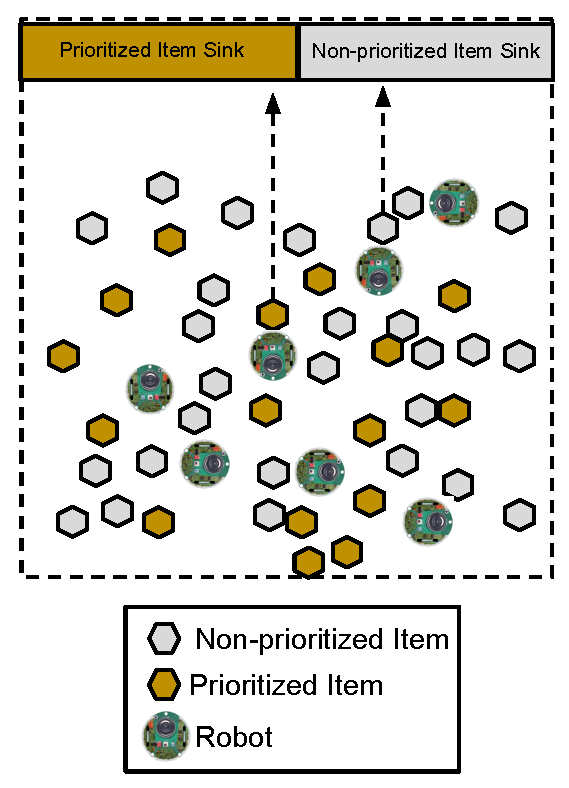
\includegraphics[width=0.65\textwidth]{chapters/chapter2/figures/EpuckGoldMining.pdf}
	\caption{Prioritized Foraging Problem }
	\label{prioritizedforaging}
\end{figure}

As per Winfield's classification described in section \ref{sec:second:taxonomy}, the prioritized foraging problem has a constrained environment, multiple source areas with multiple sinks, multiple object types, object placement is tested in a number of environment types explained in the following sections. There are multiple homogenous robots with limited sensing, relative localisation with near communications and unlimited power. Power is kept as unlimited since the energy preservation of algorithms is to be studied as a performance measure. 

%%%%%%%%%%%%%%%%%%%%%%%%%%%%%%%%%%%%%%%%%%%%%%%%%
%%%%%%%%%%%%%%%%%%%%%%%%%%%%%%%%%%%%%%%%%%%%%%%%%
\section{Summary}
\label{sec:second:summary}

%%%%%%%%%%%%%%%%%%%%%%%%%%%%%%%%%%%%%%%%%%%%%%%%%
%%%%%%%%%%%%%%%%%%%%%%%%%%%%%%%%%%%%%%%%%%%%%%%%%
%\bibliographystyle{}
%\bibliography{chapter2}